\newpage 
\pagenumbering{arabic}
\setcounter{page}{1}
%%\clearpage
\section*{Supplementary Figures}

\renewcommand{\thefigure}{S\arabic{figure}}
\setcounter{figure}{0}

\begin{figure*}[h]
\centering
\scalebox{1}{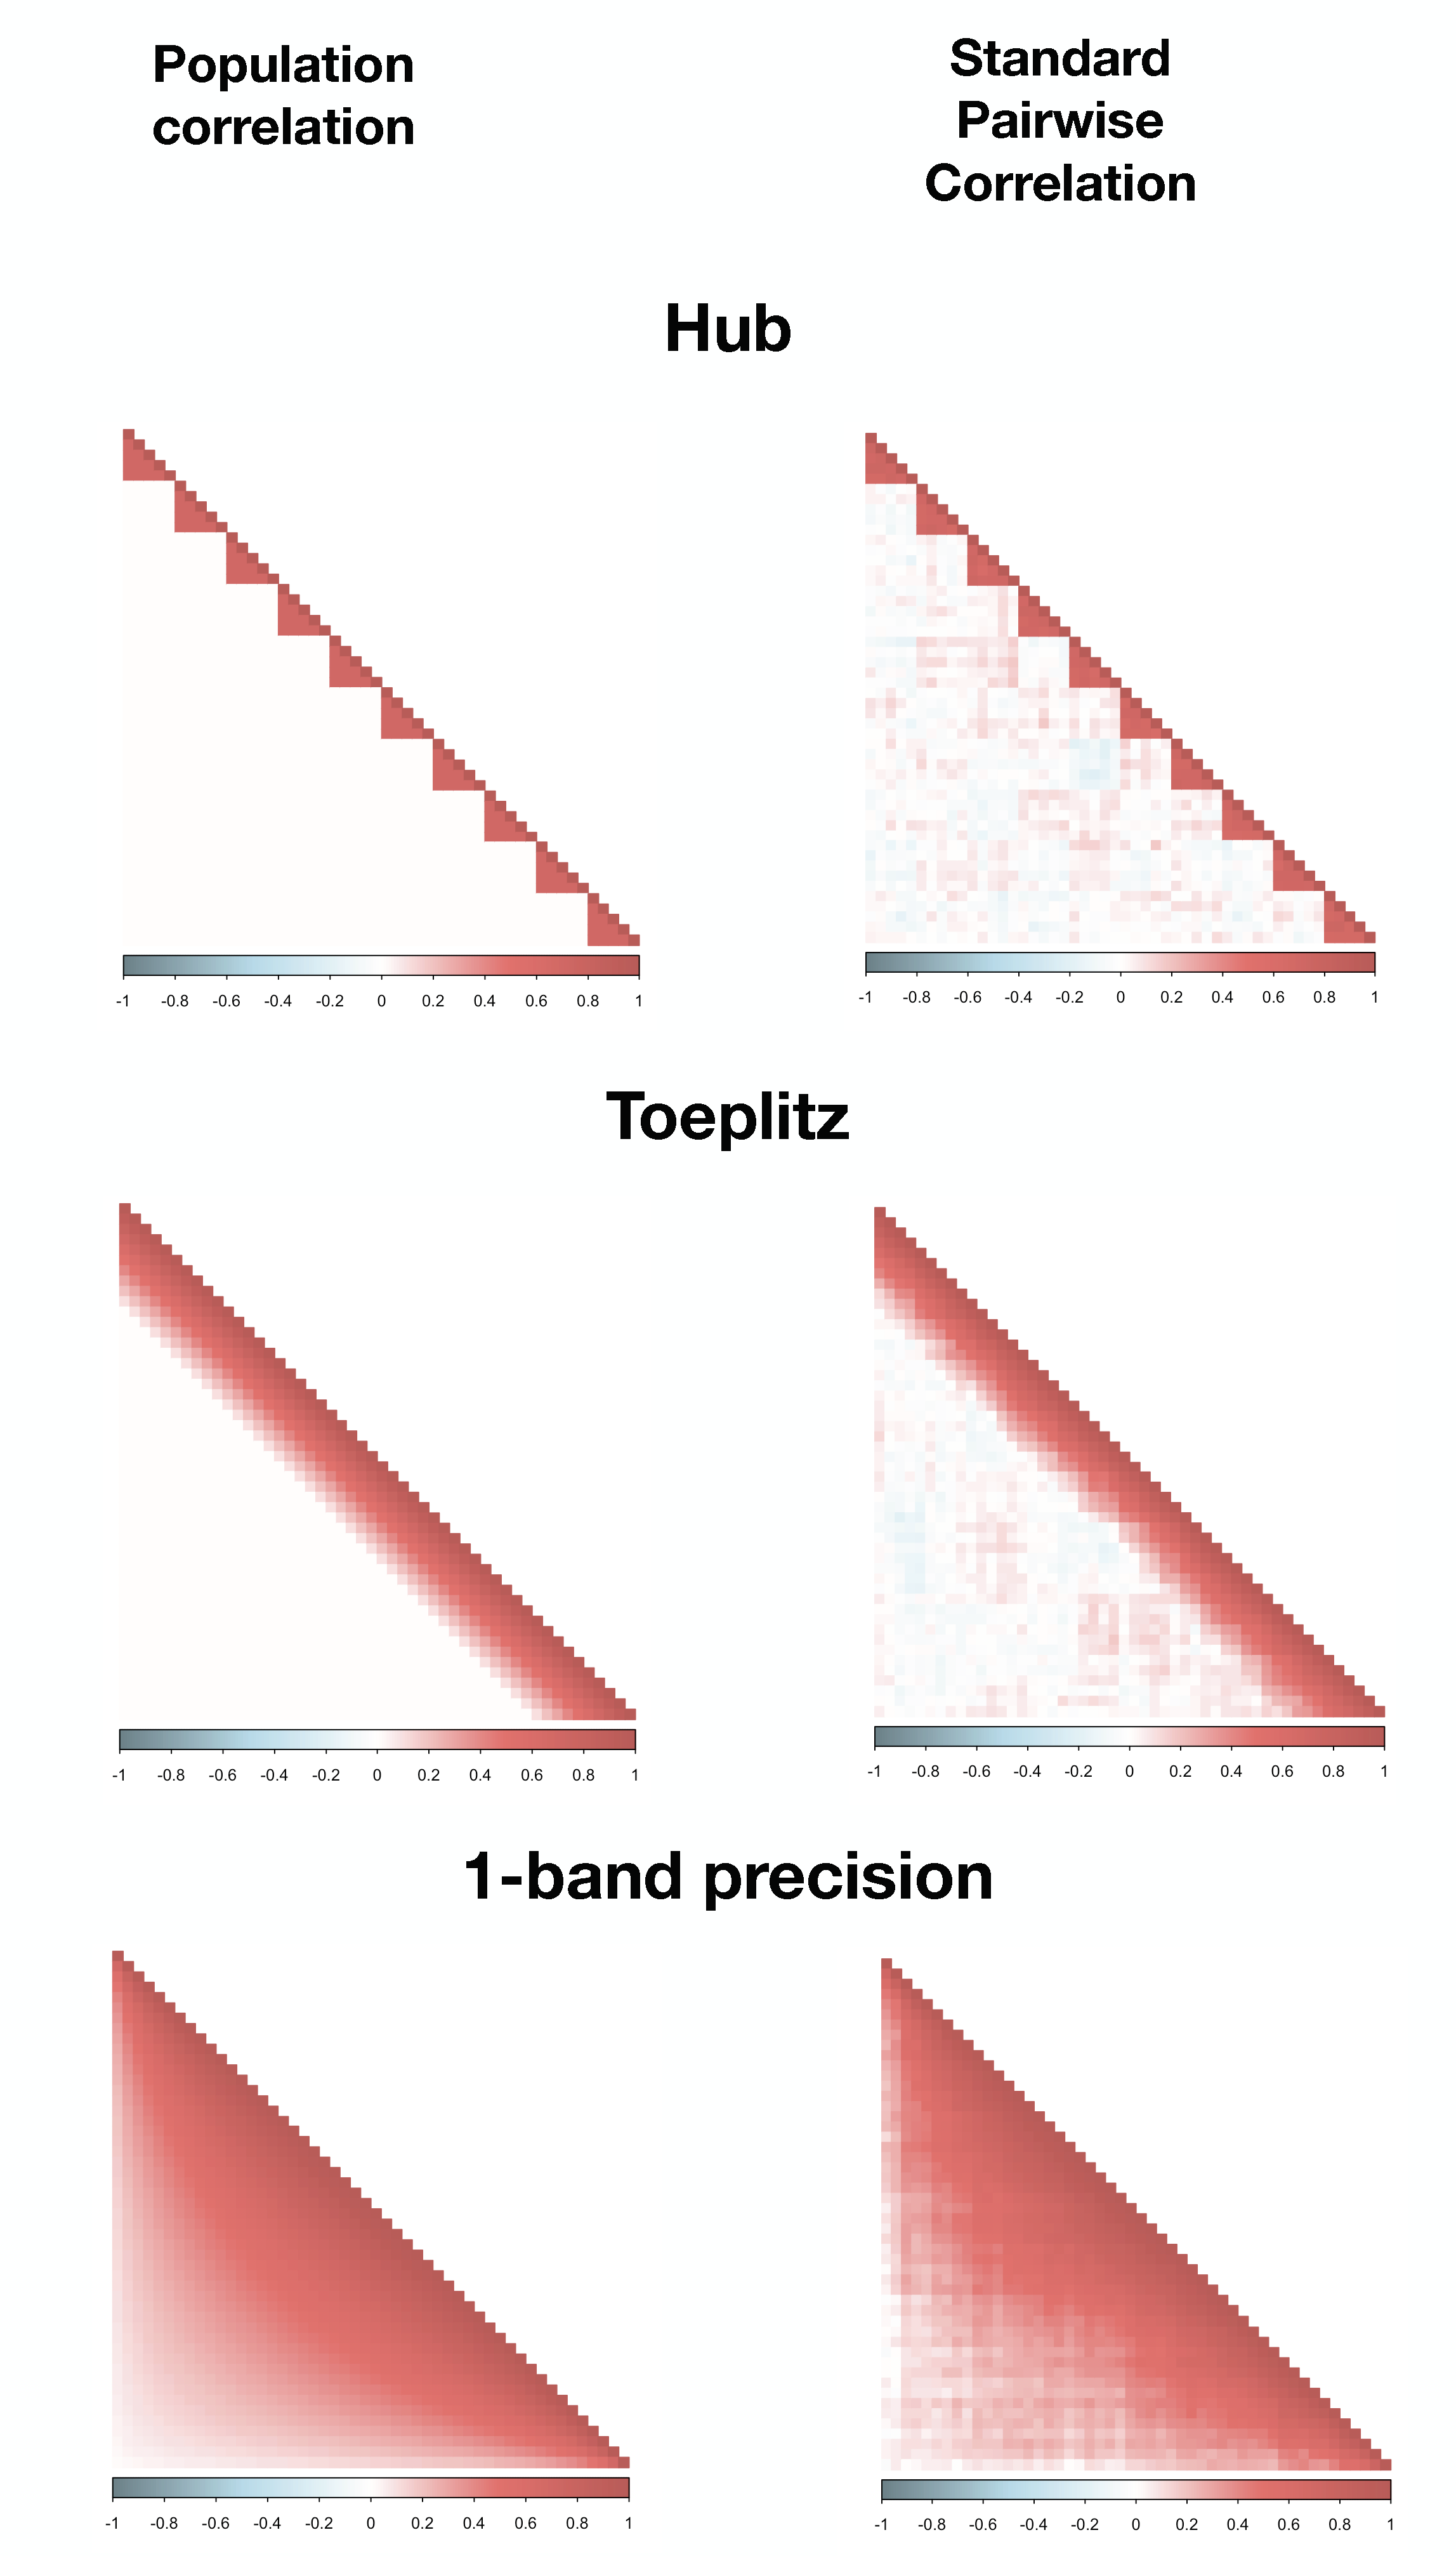
\includegraphics[ width=0.8\textwidth]{sim_standard_pop.png}}
\caption{\small We applied standard pairwise correlation estimator on data generated from the simulation models from Figure \ref{fig:sim_results}---this comprises of Hub, Toeplitz or 1-band precision matrix-based population models with 
%%$(N=500, P=50, \pi=0.5)$, representing 
$N=500$ samples, $P=50$ features and $\pi=50\%$ proportion of missing data.}
\label{fig:standard_cor_sim}
\end{figure*}



%%%\newpage

\newpage
\begin{figure*}[h]
\centering
\scalebox{1}{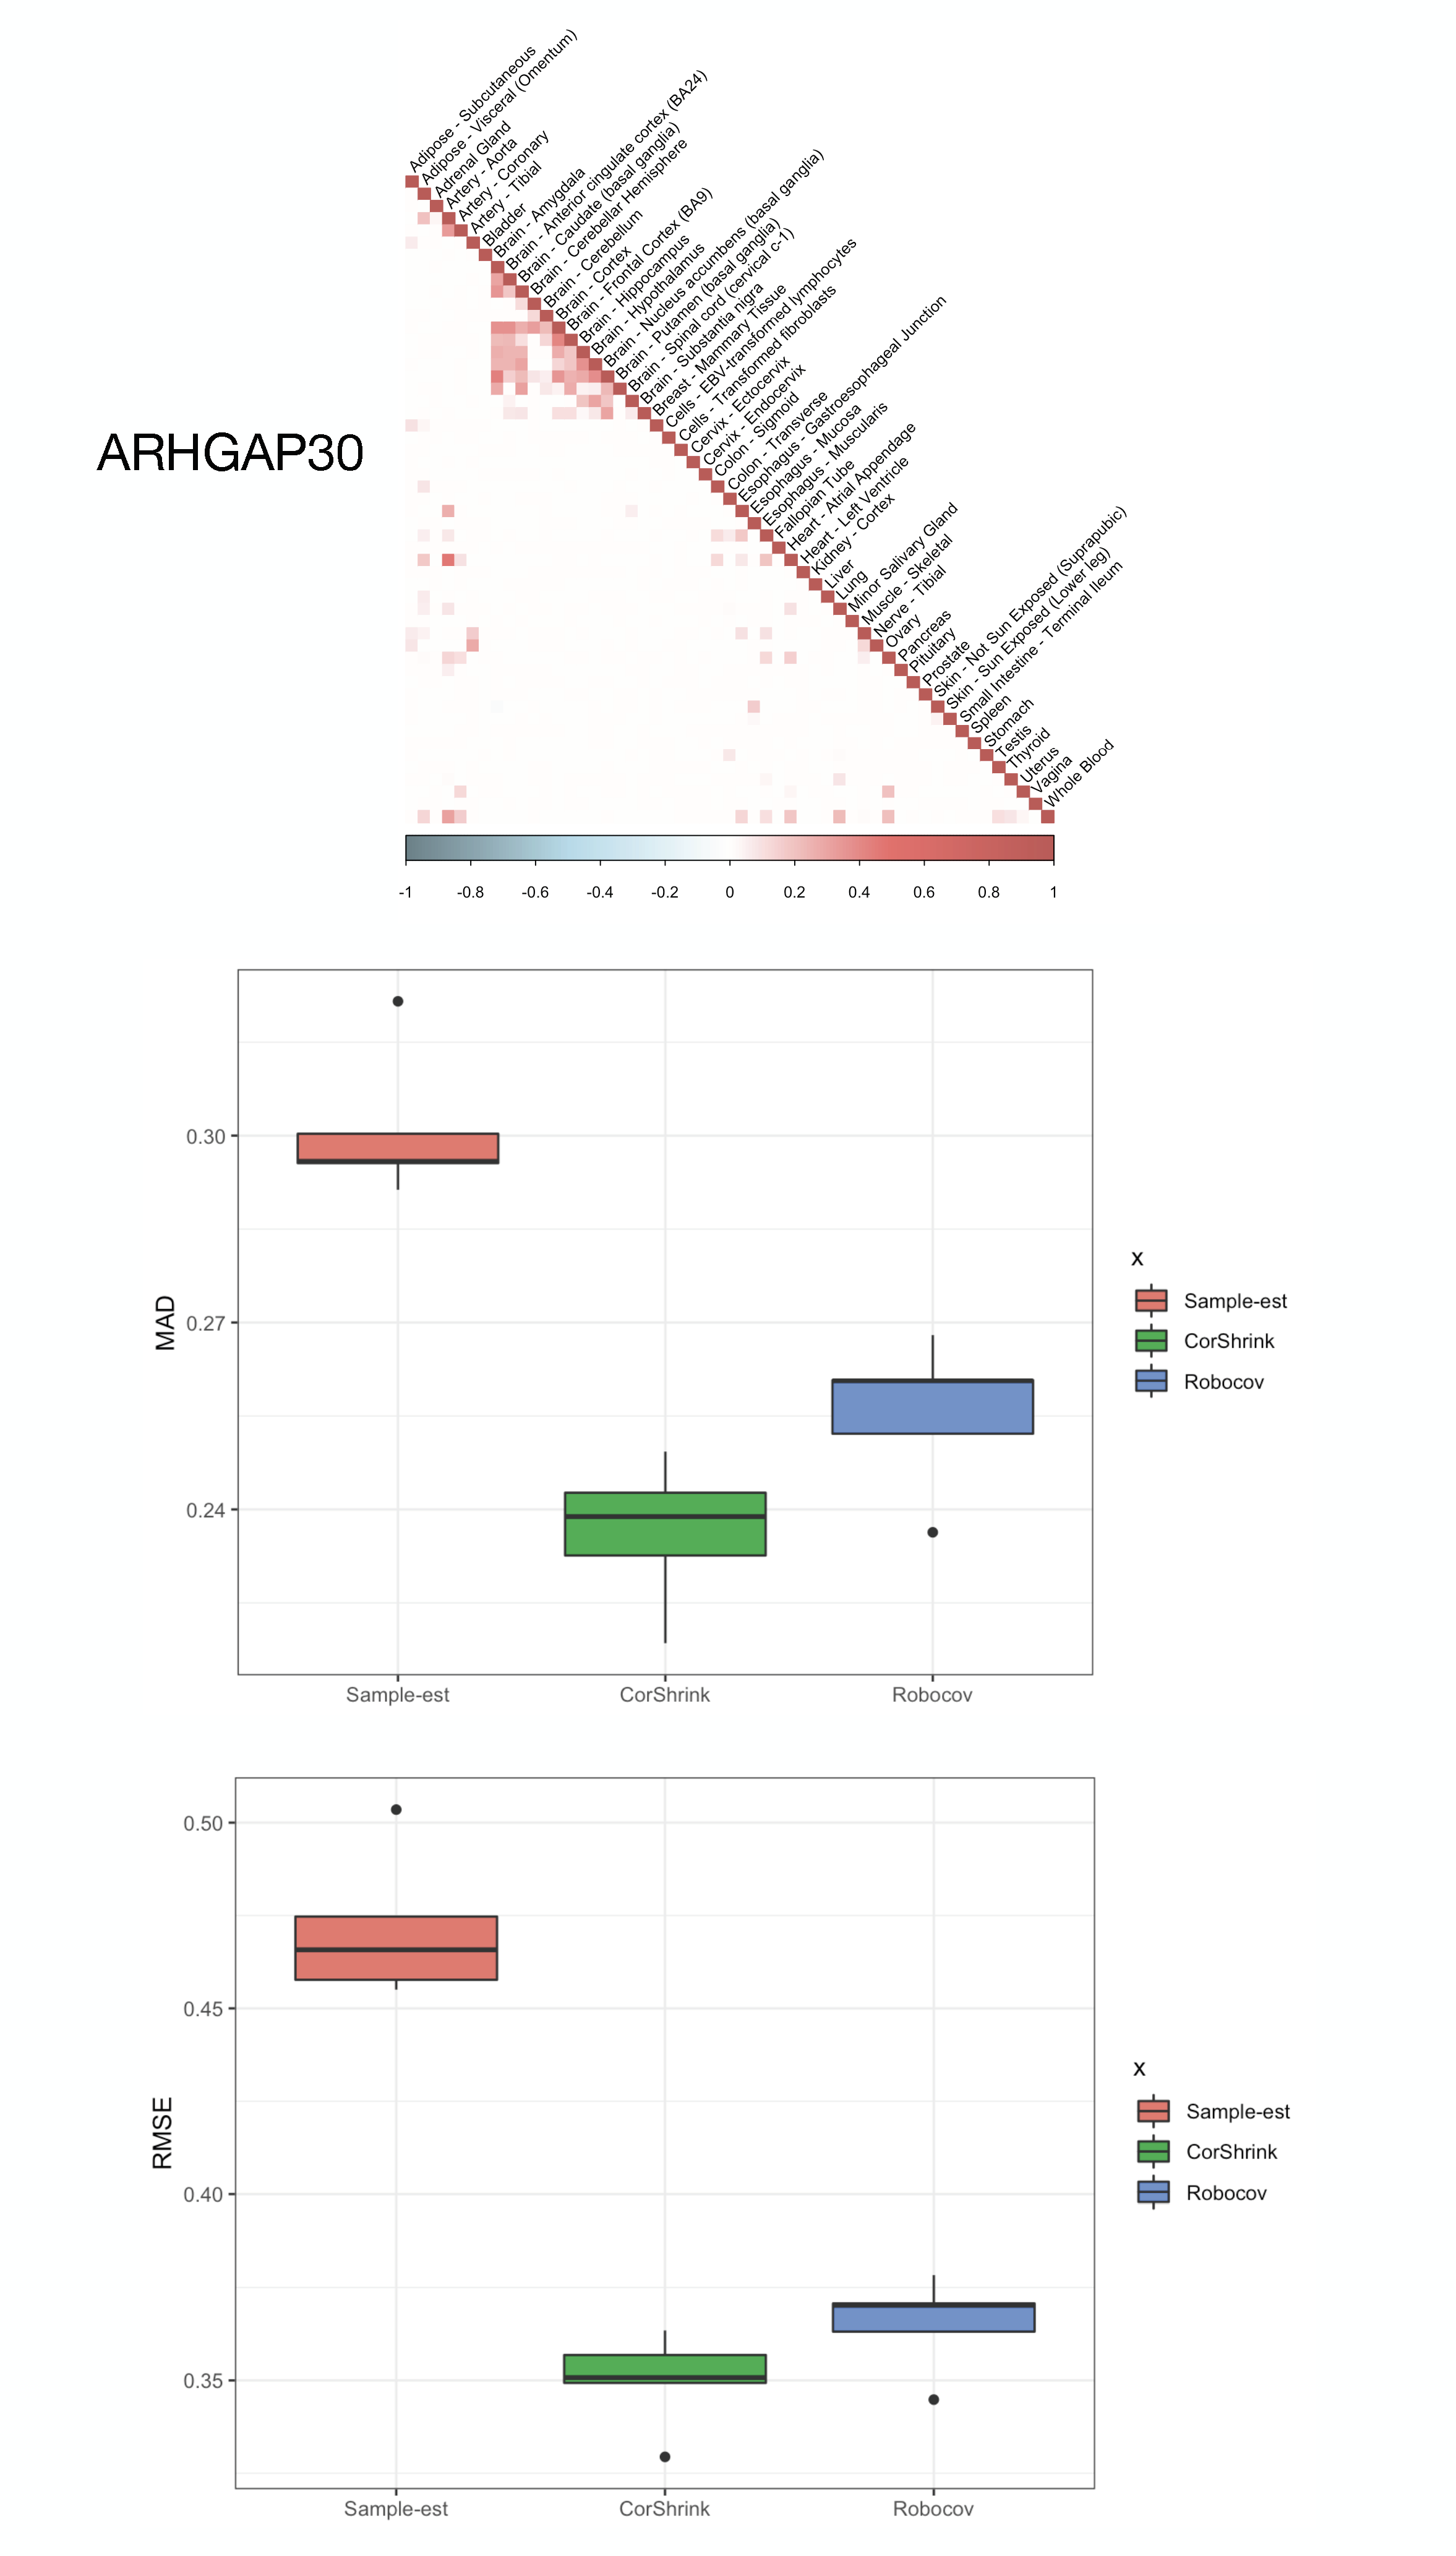
\includegraphics[ width=0.8\textwidth]{gtex_predictive.png}}
\caption{\small (Top panel) \Robocov{} correlation estimate of the \textbf{ARHGAP30} gene. (Middle and bottom panels) We split the data matrix randomly into 2 equal groups. We compare the \Robocov{}, \CorShrink{} and pairwise sample correlation estimators from one half of the data with the pairwise sample correlation matrix on the other half. We use Median Absolute Deviation (MAD) (middle panel) and Root Mean Squared Error (RMSE) (lower panel) metrics. The results are averaged over 50 such random splits. See Table \ref{tab:gtex_predictive} for a numerical summary.}
\label{fig:gtex_predictive}
\end{figure*}

\newpage

\begin{figure*}[!tpb]
\centering
\scalebox{1}{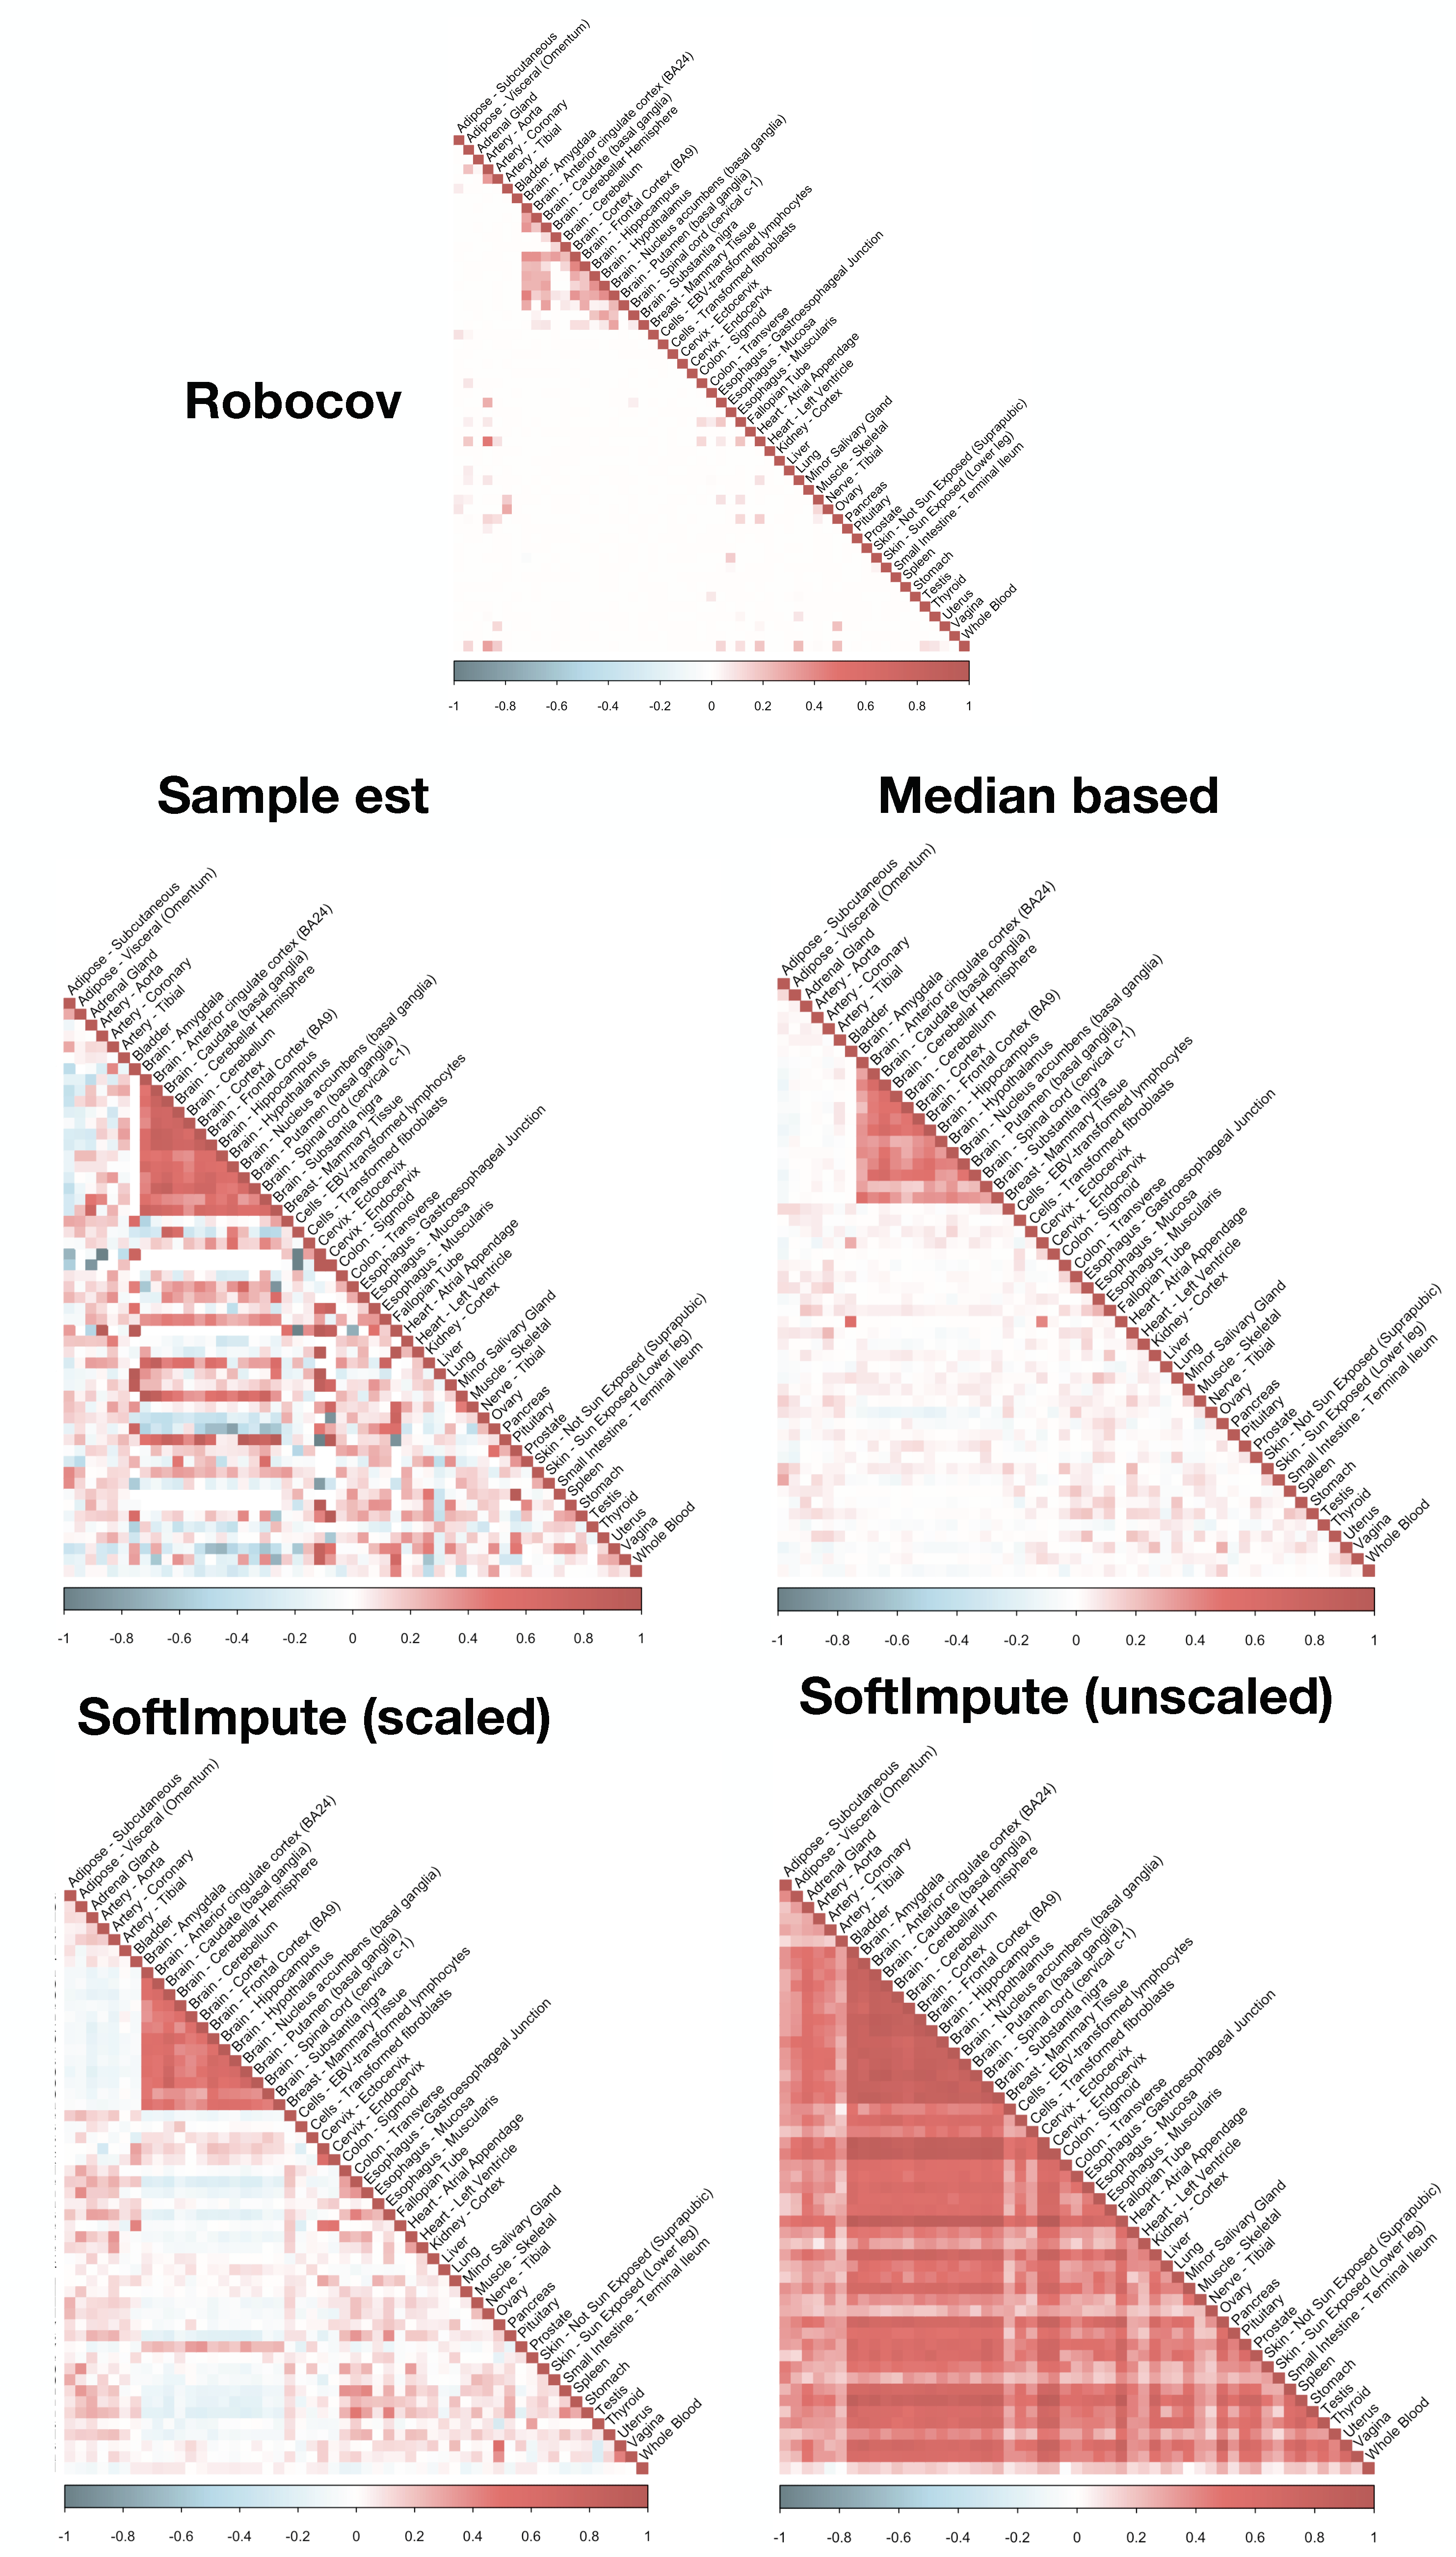
\includegraphics[ width=0.8\textwidth]{supp_non_robocov.png}}
\caption{\small We compare the \Robocov{} correlation estimator for the ARHGAP30 gene with four other estimators. They include the standard pairwise sample correlation estimator, the sample correlation matrix computed over data imputed by either a  median-based approach (missing entries of a feature replaced by the median of observed entries), the scaled SoftImpute\cite{mazumder2015} approach; and an unscaled SoftImpute\cite{mazumder2015} approach.}
\label{fig:supp_imputed}
\end{figure*}

\newpage 

\begin{figure*}[!tpb]
\centering
\scalebox{1}{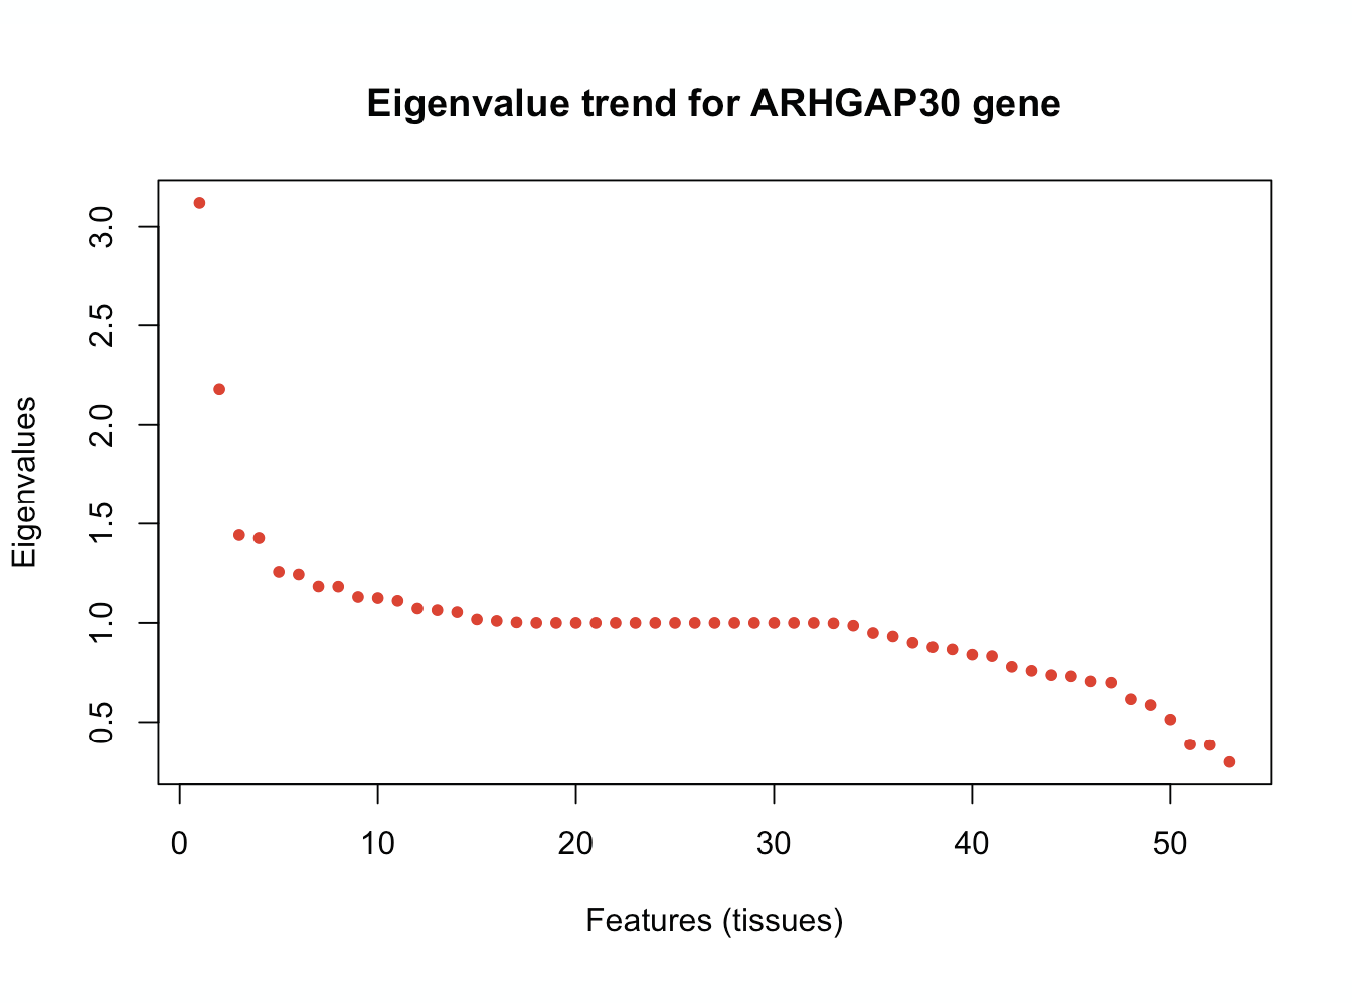
\includegraphics[ width=0.8\textwidth]{supp_highrank.png}}
\caption{\small Plot of eigenvalues sorted from highest to lowest in magnitude for tissue-tissue pairwise correlation matrix for a particular gene (ARHGAP30). The eigenvalues do not show any sharp drop close to 0 as one would expect if the matrix allowed a low rank (+noise) structure. This suggests relatively high dimensional structure in the GTEx gene expression data which may explain why a low rank imputation method such as SoftImpute\cite{mazumder2015} performs poorly in \ref{fig:supp_imputed}.}
\label{fig:gtex_highrank}
\end{figure*}


\newpage
\begin{figure*}[!tpb]
\centering
\scalebox{1}{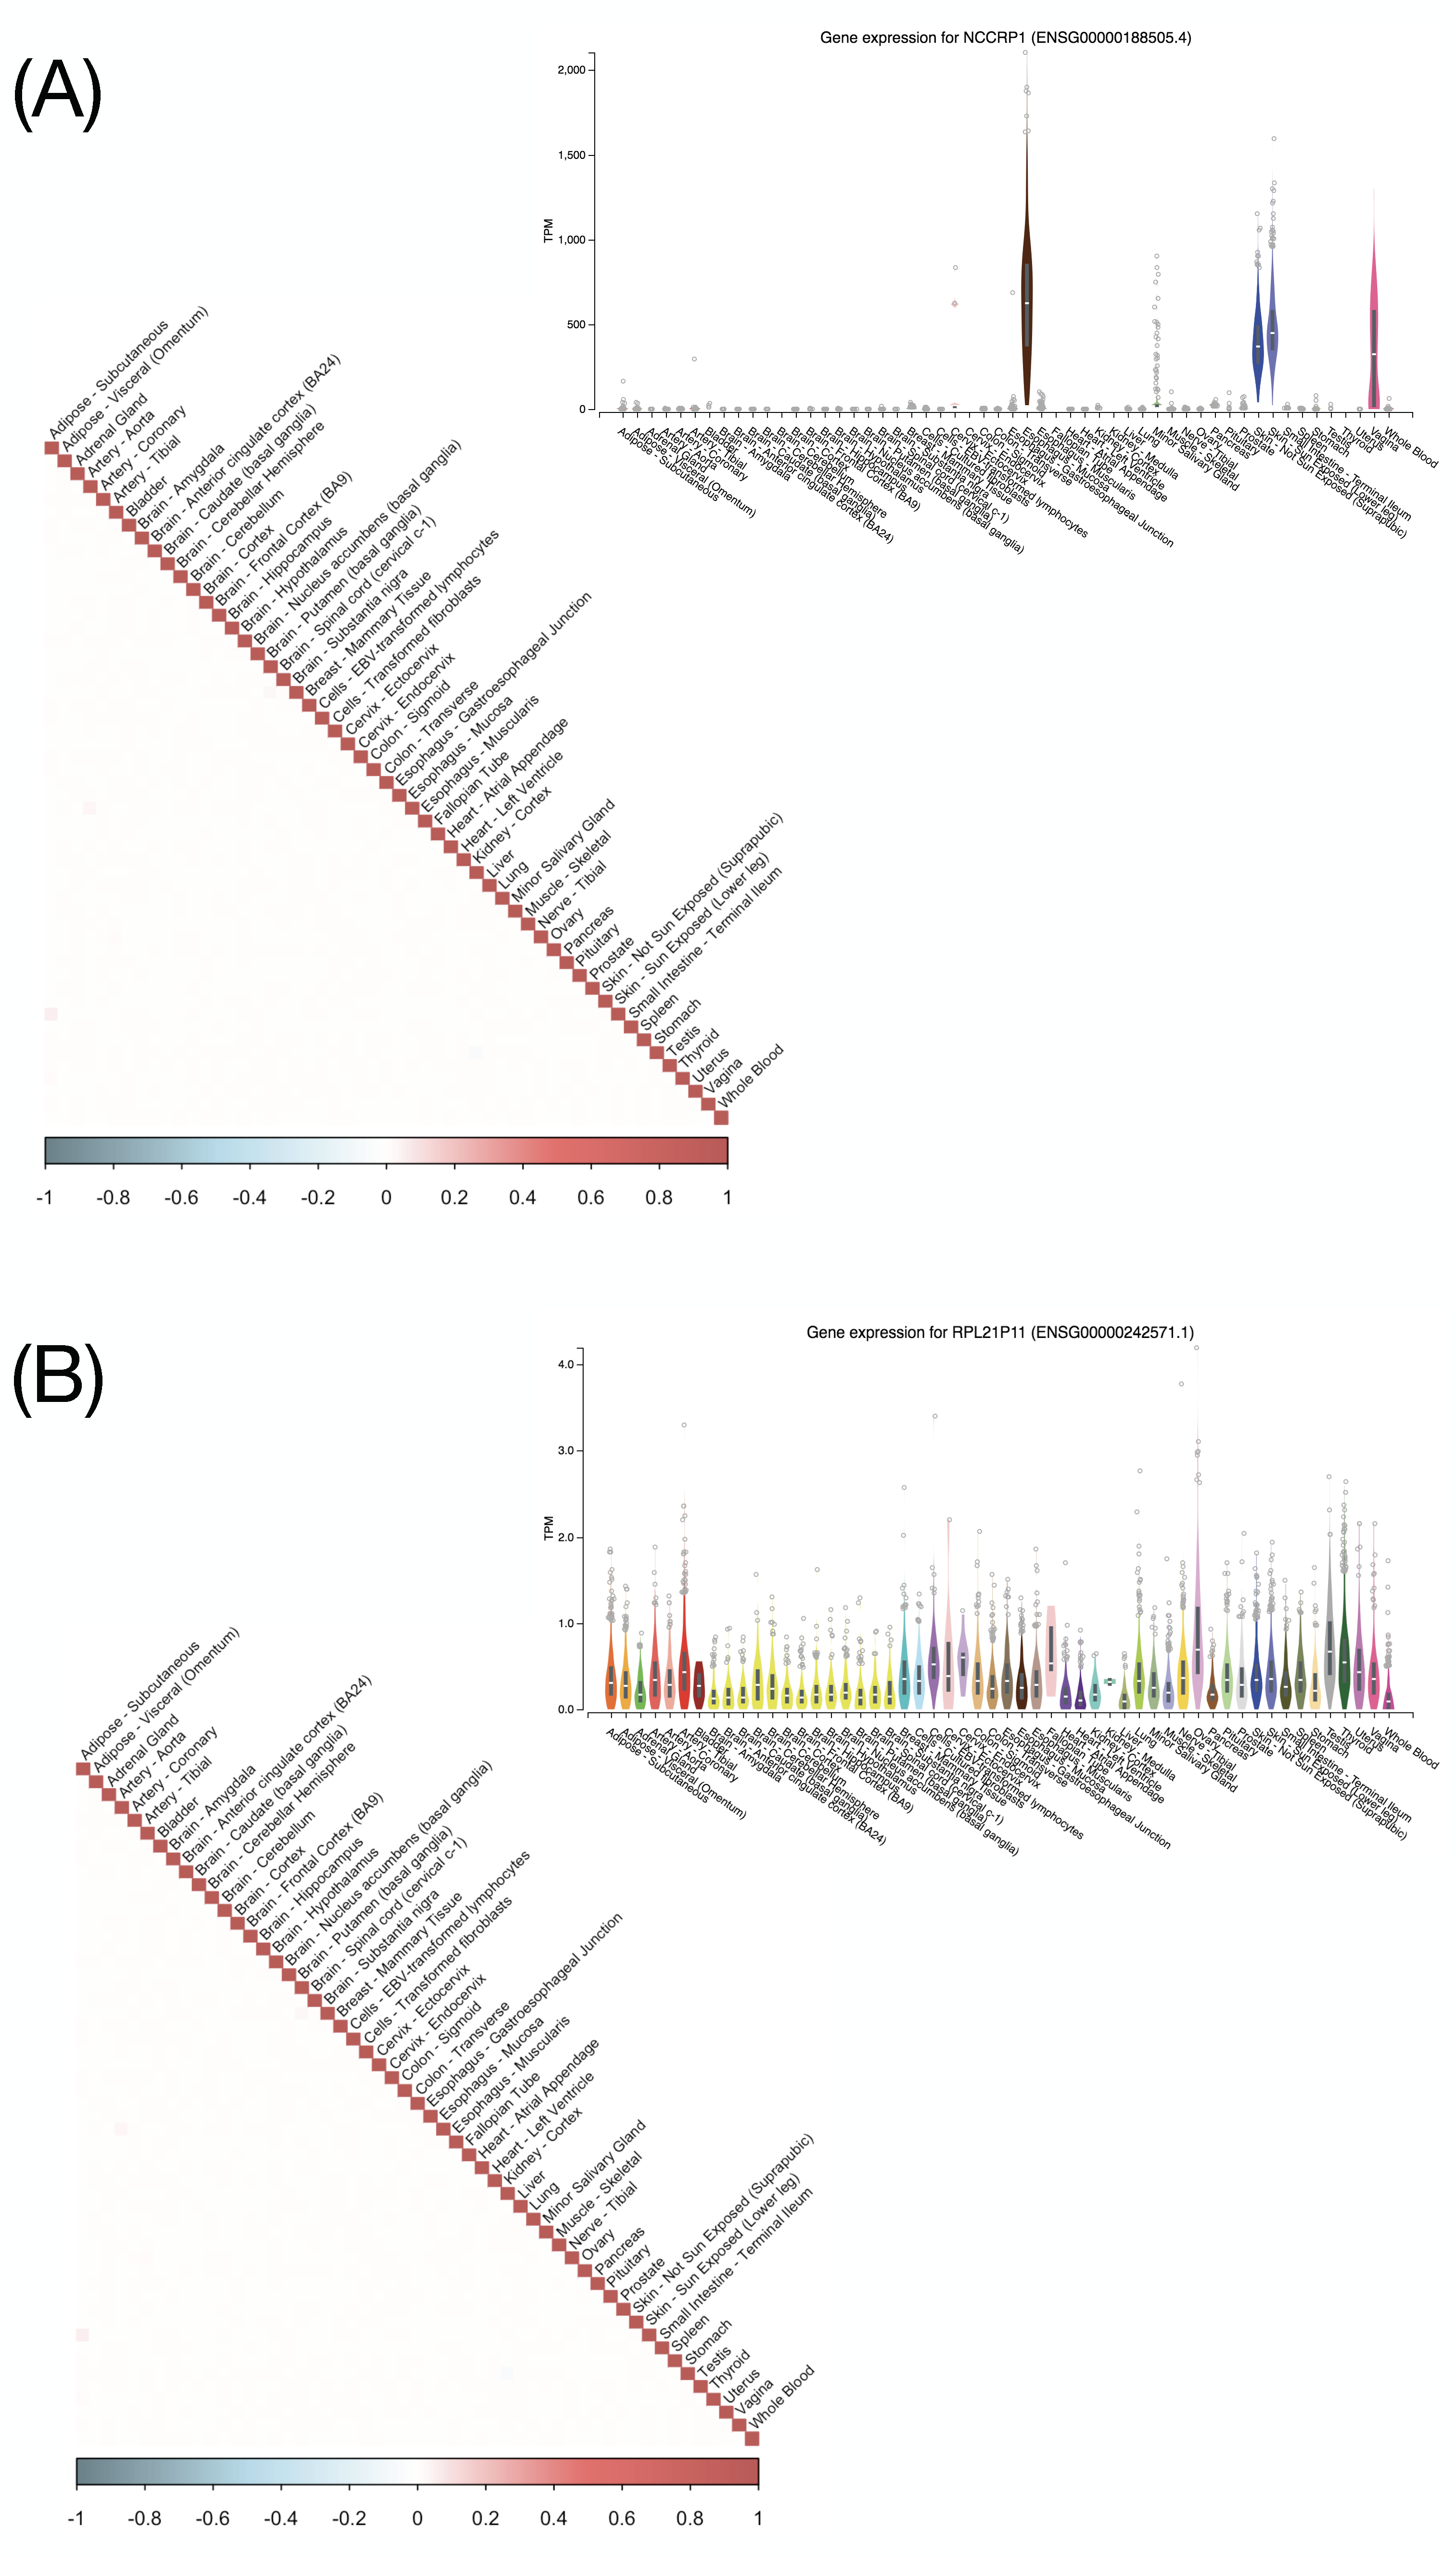
\includegraphics[height=0.8\textheight]{suppfig_gtex_examples.png}}
\caption{\small Examples of two genes, \textbf{NCCRP1} (top) and \textbf{RPL21P11} (bottom), both of which have close to 0 average correlation in expression across tissue-pairs but having very distinctive expression profiles. \textbf{NCCRP1} has high expression in a few specific tissues including Whole Blood, while \textbf{RPL21P11} has uniformly low expression across all tissues. The expression profile plots for the genes have been fetched from the GTEx Portal (\url{https://gtexportal.org/home/}).}
\label{fig:suppfig_gtex_examples}
\end{figure*}

\newpage
\begin{figure*}[!tpb]
\centering
\scalebox{1}{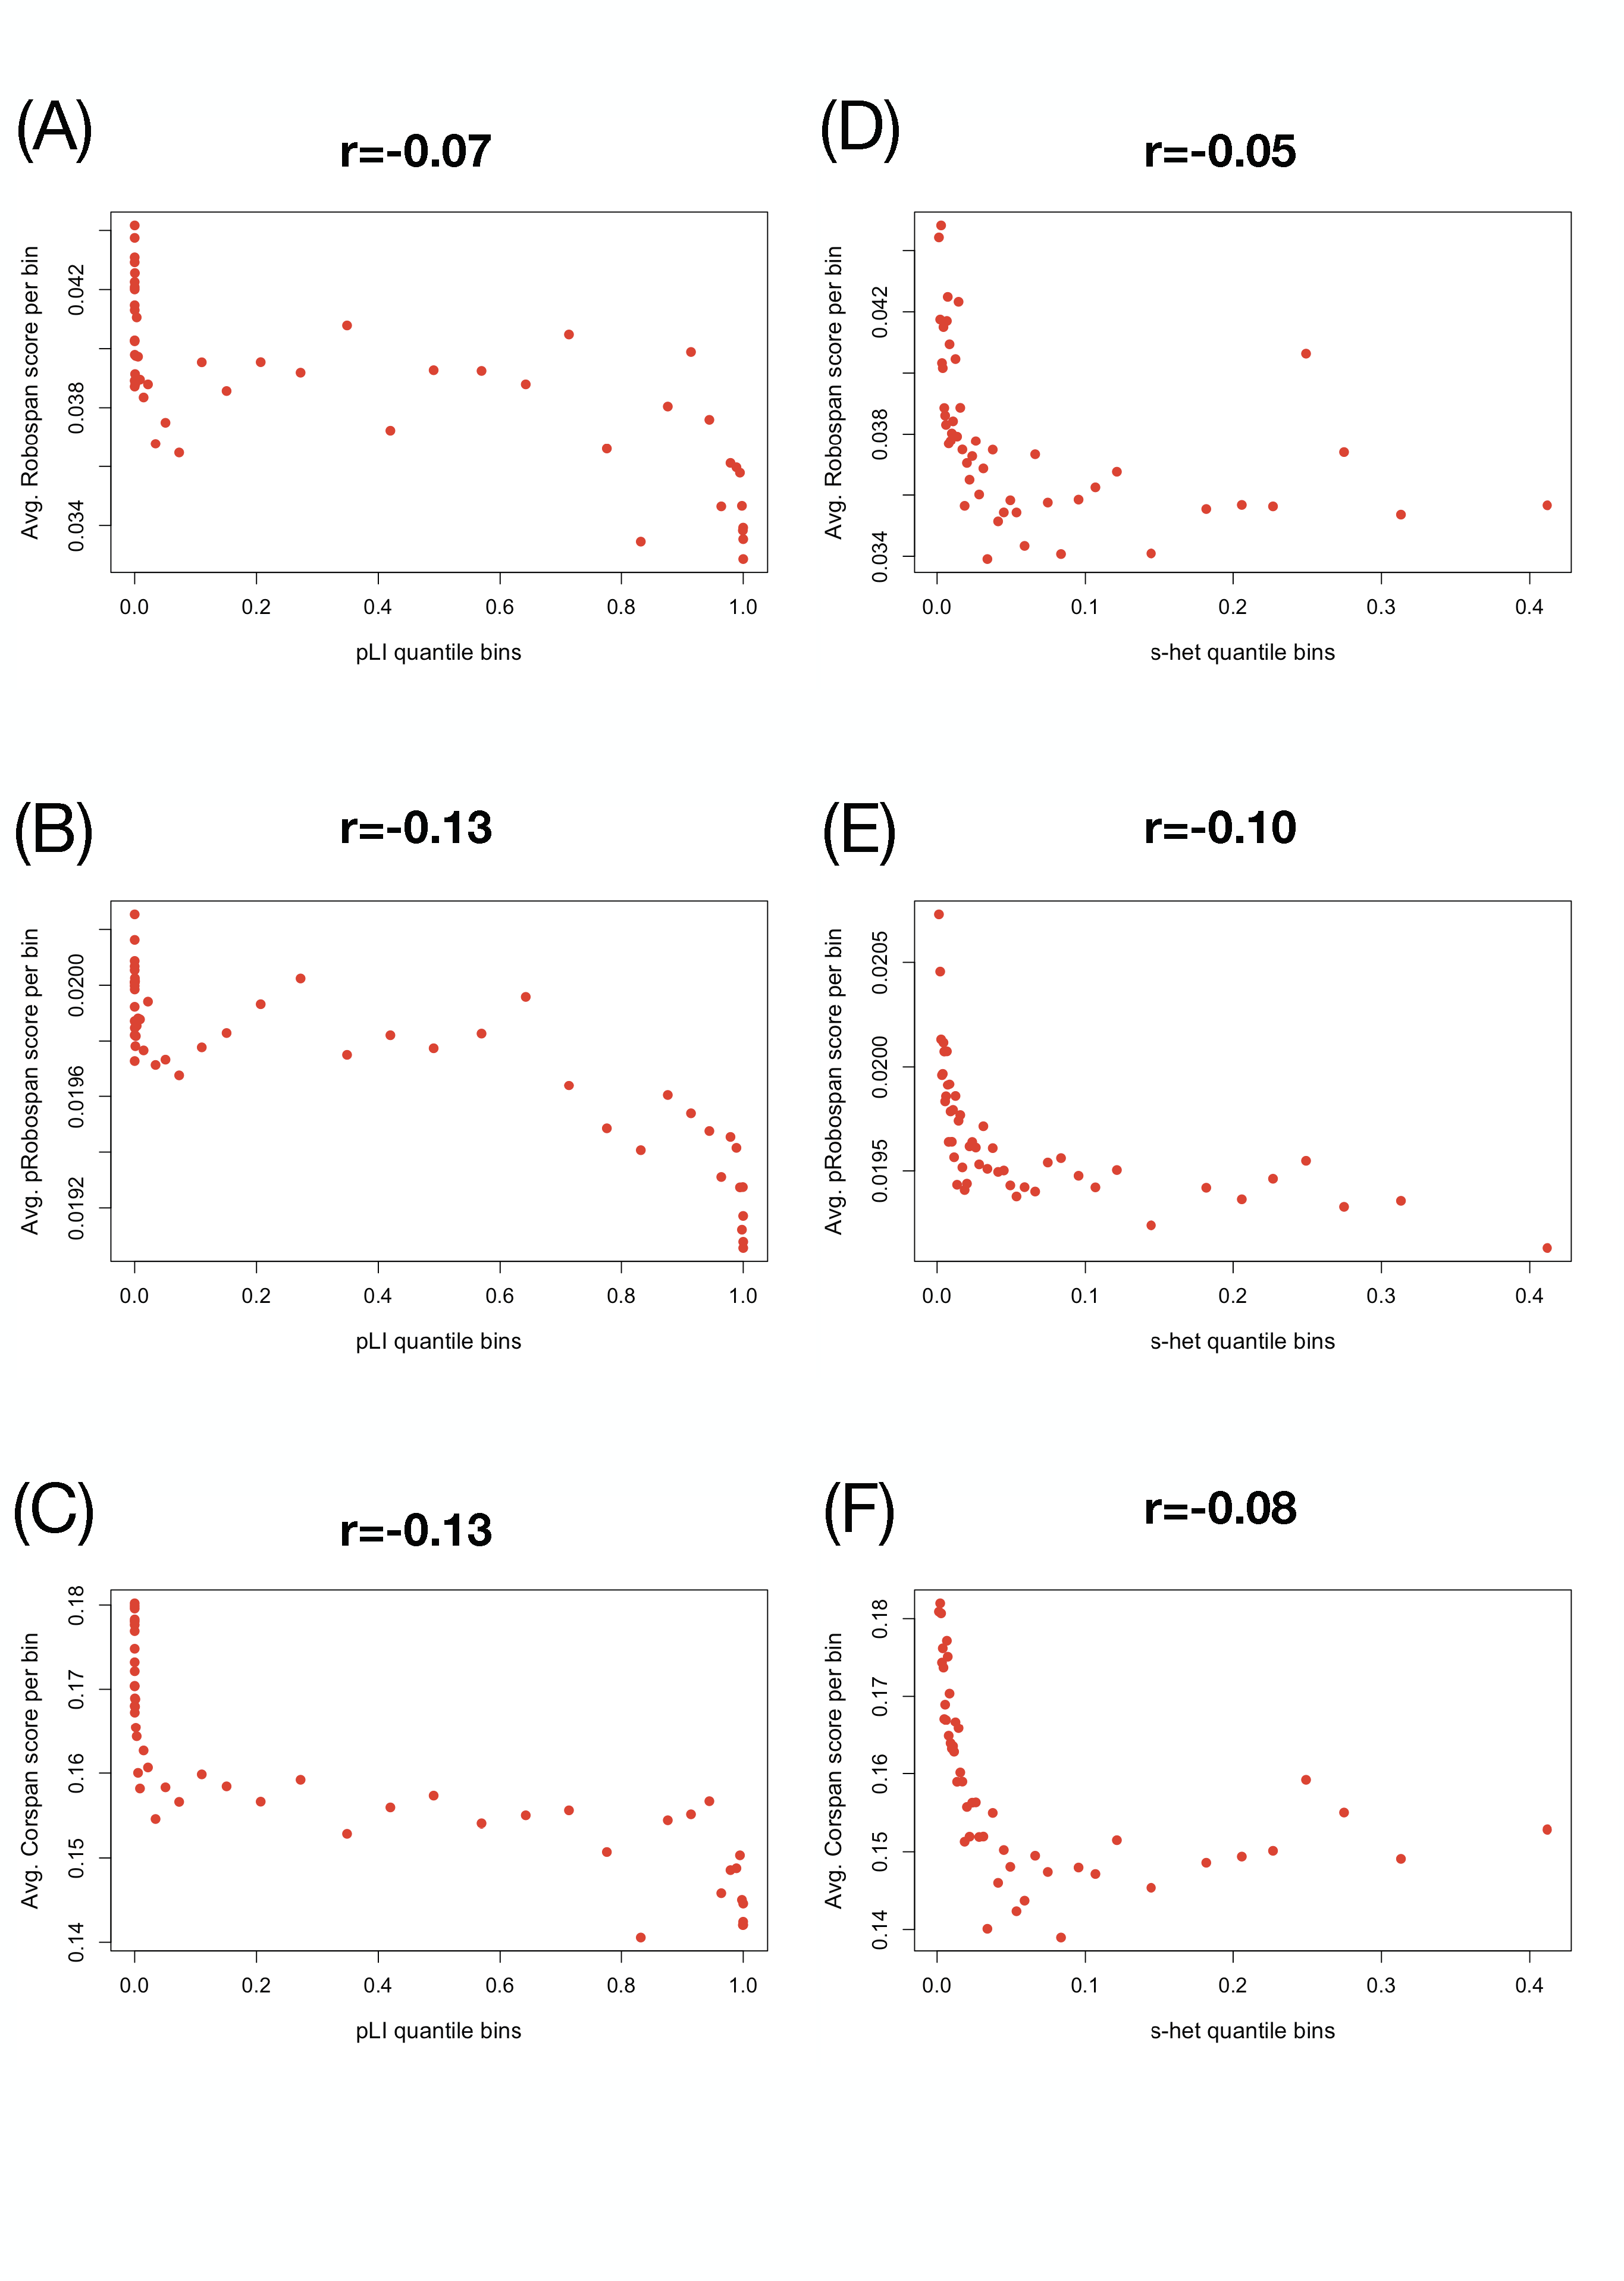
\includegraphics[height=0.8\textheight]{pLI_shet.png}}
\caption{\small Comparison of pLI gene score with (A) Robospan-score, (B) pRobospan-score and (C) Corspan-score for all genes (See Results section for details). Comparison of s\_het gene score with (A) Robospan-score, (B) pRobospan-score and (C) Corspan-score for all genes (See Results section for details).}
\label{fig:pLI_shet}
\end{figure*}


\newpage
\begin{figure*}[!tpb]
\centering
\scalebox{1}{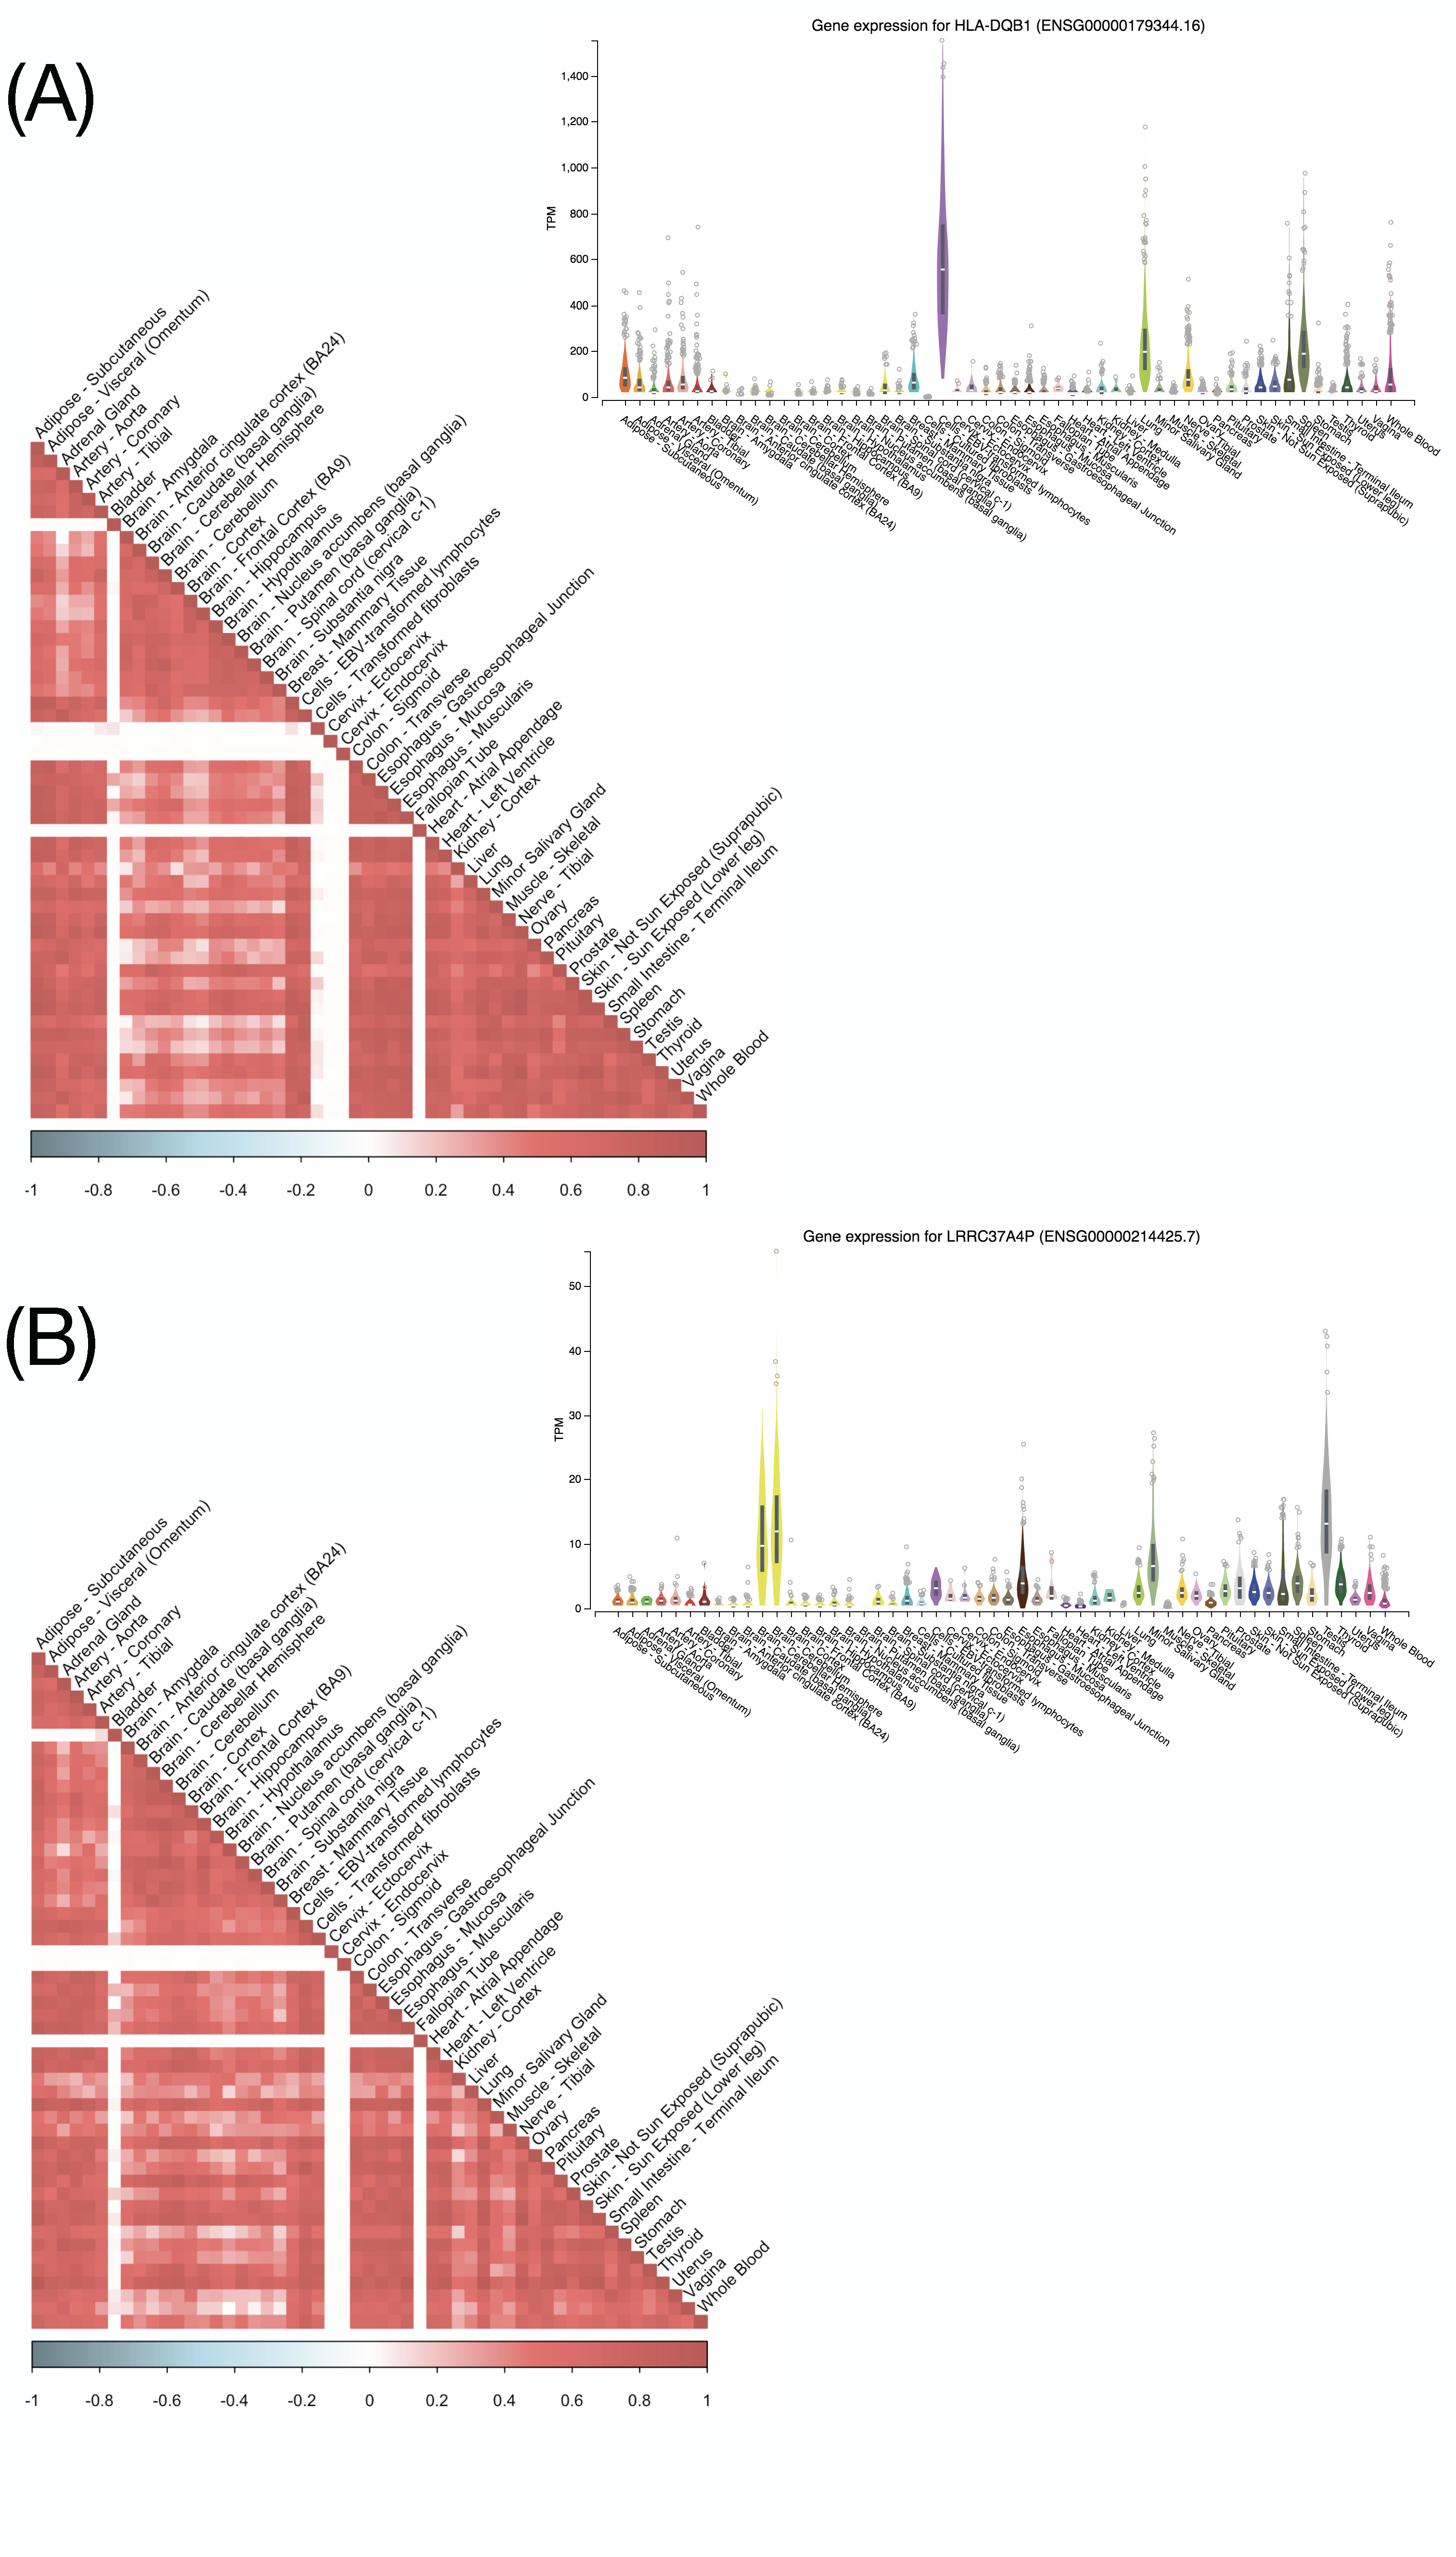
\includegraphics[height=0.8\textheight]{suppfig_gtex_examples_2.png}}
\caption{\small Examples of genes high Robospan-score but not specifically expressed in blood or uniformly expressed across tissues. The two genes are \textbf{HLA-DQB1} (top) and \textbf{LRRC37A4P} (bottom). \textbf{HLA-DQB1} is specifically expressed in lymphocyte cell line which is related to blood. \textbf{LRRC37A4P} has highest expression in brain cerebellum and testis. The expression profile plots for the genes have been fetched from the GTEx Portal (\url{https://gtexportal.org/home/}).}
\label{fig:suppfig_gtex_examples_2}
\end{figure*}

\newpage
\begin{figure*}[!tpb]
\centering
\scalebox{1}{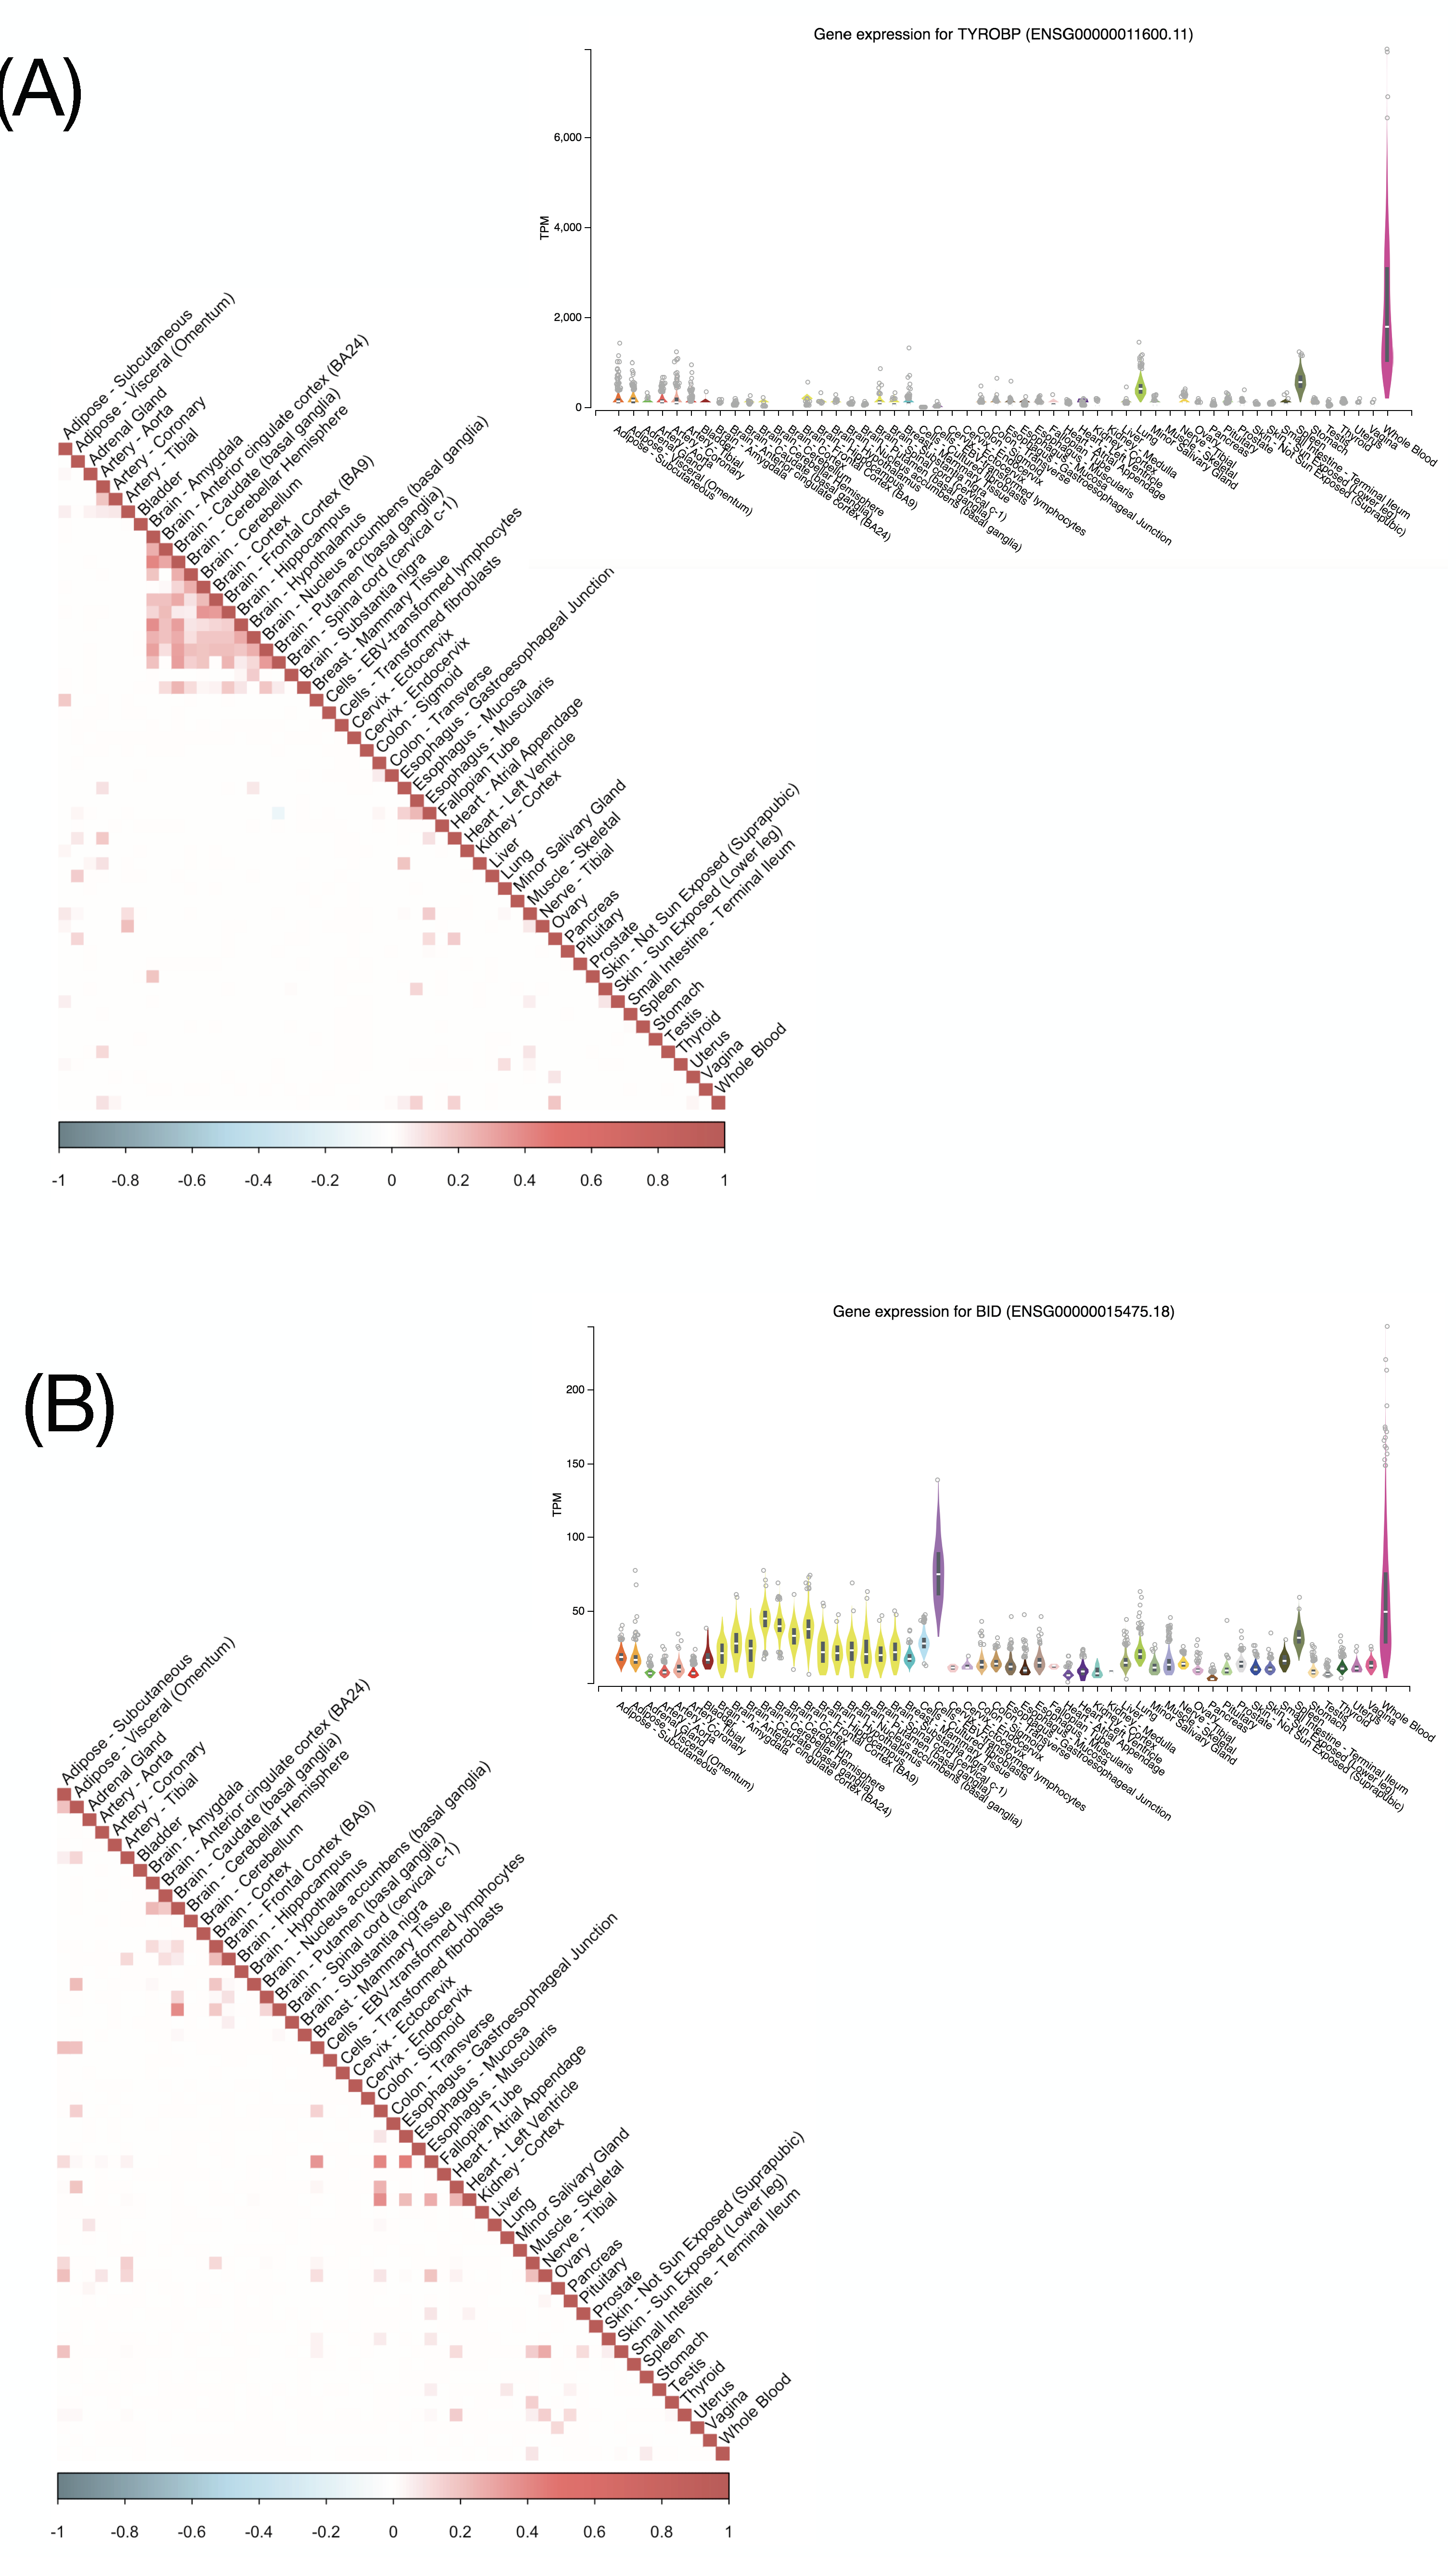
\includegraphics[height=0.8\textheight]{suppfig_gtex_examples_3.png}}
\caption{\small Examples of genes that are specifically expressed in Whole Blood but do not show high Robospan-score. The two gene are \textbf{TYROBP} (top) and \textbf{BID} (bottom). They show tissue specific expression in Whole blood and are in top 10\% specifically expressed genes (SEG) as per ref.\cite{Finucane2018}, but do not show consistently high expression correlation across tissue pairs and hence, do not have high Robospan score. The expression profile plots for the genes have been fetched from the GTEx Portal (\url{https://gtexportal.org/home/}).}
\label{fig:suppfig_gtex_examples_3}
\end{figure*}


